\documentclass[../main.tex]{subfiles}
\graphicspath{{\subfix{../figures/}}}

\begin{document}
The first step towards simulating the dynamics of the parallel quantum dot system was to calculate the matrix representation of the Liouvillian. This was done numerically using an already implemented PERLind approach to calculate the four jump operators $\hat L_i$, $i\in\{1,2,3,4\}$, each associated with one of the tunneling processes of the system (should I explain which jump operator corresponds with what tunneling process?). The total Liouvillian could then be constructed and compared with the Python-based QmeQ package (\cite{qmeq}) as a sanity check. Then, the parameter space was searched for exceptional points by numerically calculating the eigenvalues of $L$ for varying $\delta\epsilon$ and $\delta\Gamma$. A degeneracy of eigenvalues was found at $\lambda_5 = \lambda_6\approx -0.5\Gamma$, for $\delta\Gamma = 10^{-6}\Gamma$ and $\delta\epsilon \approx 0.3\Gamma$, see \cref{fig:tuning}. The corresponding eigenvectors, $\ket{\rho_5}\rangle$ and $\ket{\rho_6}\rangle$, was found to also coalesce, confirming the existence of an exceptional point. The eigenvalue and the left and right eigenvector corresponding to the EP will be denoted by $\bar \lambda$, $\langle\bra{\bar\sigma}$, and $\ket{\bar\rho}\rangle$ respectively.
\begin{figure}[H]
    \centering
    \includegraphics[width=0.9\linewidth]{figures/tuning.png}
    \caption{The real and imaginary part of two eigenvalues to $L$, $\lambda_5$ and $\lambda_6$, for varying $\delta\epsilon$. An eigenvalue degeneracy at can be seen at $\delta\epsilon\approx0.3\Gamma$.}
    \label{fig:tuning}
\end{figure}

The full spectrum of the Liouvillian at the exceptional point is given in \cref{fig:spec}, where the eigenvalue degeneracy between $\lambda_5$ and $\lambda_6$ is clear. There is almost a degeneracy between $\lambda_3$ and $\lambda_4$, however, this is not a second EP since the eigenvectors are not parallel. Furthermore, note that all eigenvalues are on the negative real axis, indicating exponential decay towards the steady-state in the dynamics of the system. 
\begin{figure}[H]
    \centering
    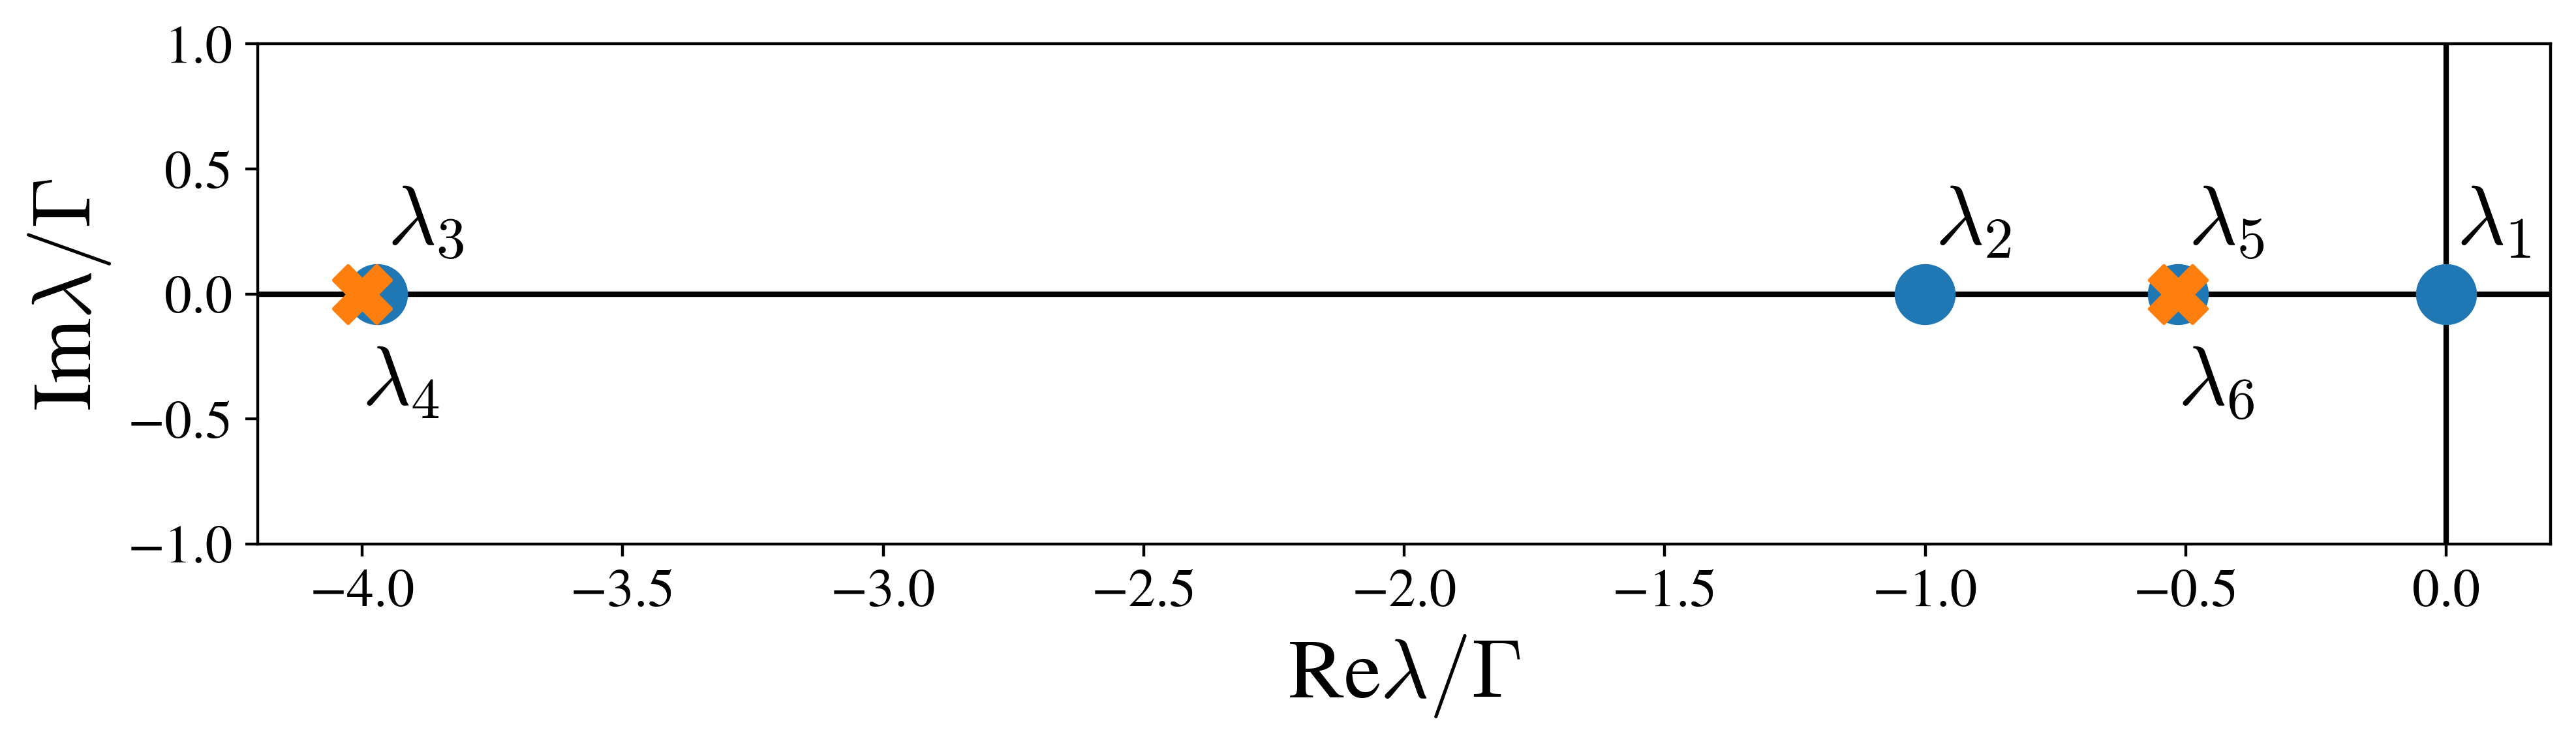
\includegraphics[width=0.8\linewidth]{figures/spectrum.png}
    \caption{The spectrum of the Liouvillian at the exceptional point. The crosses are used to distinguish eigenvalues which are close to each other.}
    \label{fig:spec}
\end{figure}

Using \cref{eq:genmode}, the evolution of the system can be given in terms of the eigenvalues and generalized eigenvectors of $L$. Away from an exceptional point, the Liouvillian is diagonalizable, and the terms are purely exponential. The evolution of the density operator is then given by
\begin{equation}\label{eq:dynnonep}
    \ket{\rho(t)}\rangle = \ket{\rho_{ss}}\rangle + \sum_{i=2}^6 c_i e^{\lambda_i t} \ket{\rho_i}\rangle
\end{equation}
where $\ket{\rho_i}\rangle$ is the $i$th right eigenvector of $L$, and $c_i = \langle\braket{\sigma_i|\rho(0)}\rangle$. Here, $\langle\bra{\sigma_i}$ is the $i$th left eigenvector, constructed biorthogonally to $\ket{\rho_i}\rangle$. Furthermore, $\ket{\rho_{ss}}\rangle = c_1 \ket{\rho_1}\rangle$ is the steady state of the system, due to the zero eigenvalue $\lambda_1=0$.

At the exceptional point, the Jordan form of $L$ and its exponential $e^{Jt}$ have to be evaluated. Since the EP is of order two, this results in a $2\times2$ Jordan block. This is the only EP, which means that rest of the Jordan form is diagonal. Using \cref{eq:jordan,eq:expjordan}, this results in the following Jordan form and Jordan exponential:

\begin{equation}
    J = \begin{bmatrix} 0 & 0 & 0 & 0 & 0 & 0 \\
                        0 & \lambda_2 & 0 & 0 & 0 & 0 \\
                        0 & 0 & \lambda_3 & 0 & 0 & 0 \\
                        0 & 0 & 0 & \lambda_4 & 0 & 0 \\
                        0 & 0 & 0 & 0 & \bar \lambda & 1 \\
                        0 & 0 & 0 & 0 & 0 & \bar \lambda \\ \end{bmatrix}, \; 
        e^{Jt} = \begin{bmatrix} 1 & 0 & 0 & 0 & 0 & 0 \\
            0 & e^{\lambda_2t} & 0 & 0 & 0 & 0 \\
            0 & 0 & e^{\lambda_3t} & 0 & 0 & 0 \\
            0 & 0 & 0 & e^{\lambda_4t} & 0 & 0 \\
            0 & 0 & 0 & 0 & e^{\bar \lambda t} & t \\
        0 & 0 & 0 & 0 & 0 & e^{\bar \lambda t} \\ \end{bmatrix},
\end{equation}
since $\lambda_1 = 0$.

Furthermore, the Jordan chain vector, here written as $\ket{\rho'}\rangle$, defined by $(L - \bar\lambda I)\ket{\rho'}\rangle = \ket{\bar\rho}\rangle$ and the corresponding left generalized eigenvector $\langle\bra{\sigma'}$, need to be evaluated. Inserting these vectors into \cref{eq:genmode}, the evolution of the density operator can be shown to be given by
\begin{equation}\label{eq:dynep}
    \begin{aligned}
        \ket{\rho(t)}\rangle = \ket{\rho_{ss}}\rangle + \sum_{i=2}^4 c_i e^{\lambda_i t} \ket{\rho_i}\rangle  
                                + (\bar c + c't)e^{\bar \lambda t}\ket{\bar \rho}\rangle + c'e^{\bar\lambda t}\ket{\rho'}\rangle,
    \end{aligned}
\end{equation}
where $\bar c = \langle\braket{\bar\sigma|\rho(0)}\rangle$, and $c' = \langle\braket{\sigma'|\rho(0)}\rangle$.

By numerically calculating the generalized eigenvectors as described in \cref{sec:jordan}, the dynamics at non-EP and at EP given by \cref{eq:dynnonep,eq:dynep}, could be implemented. The results were then compared with a numerical ODE-solver, see \cref{fig:minevsint}.

\begin{figure}[H]
    \centering
    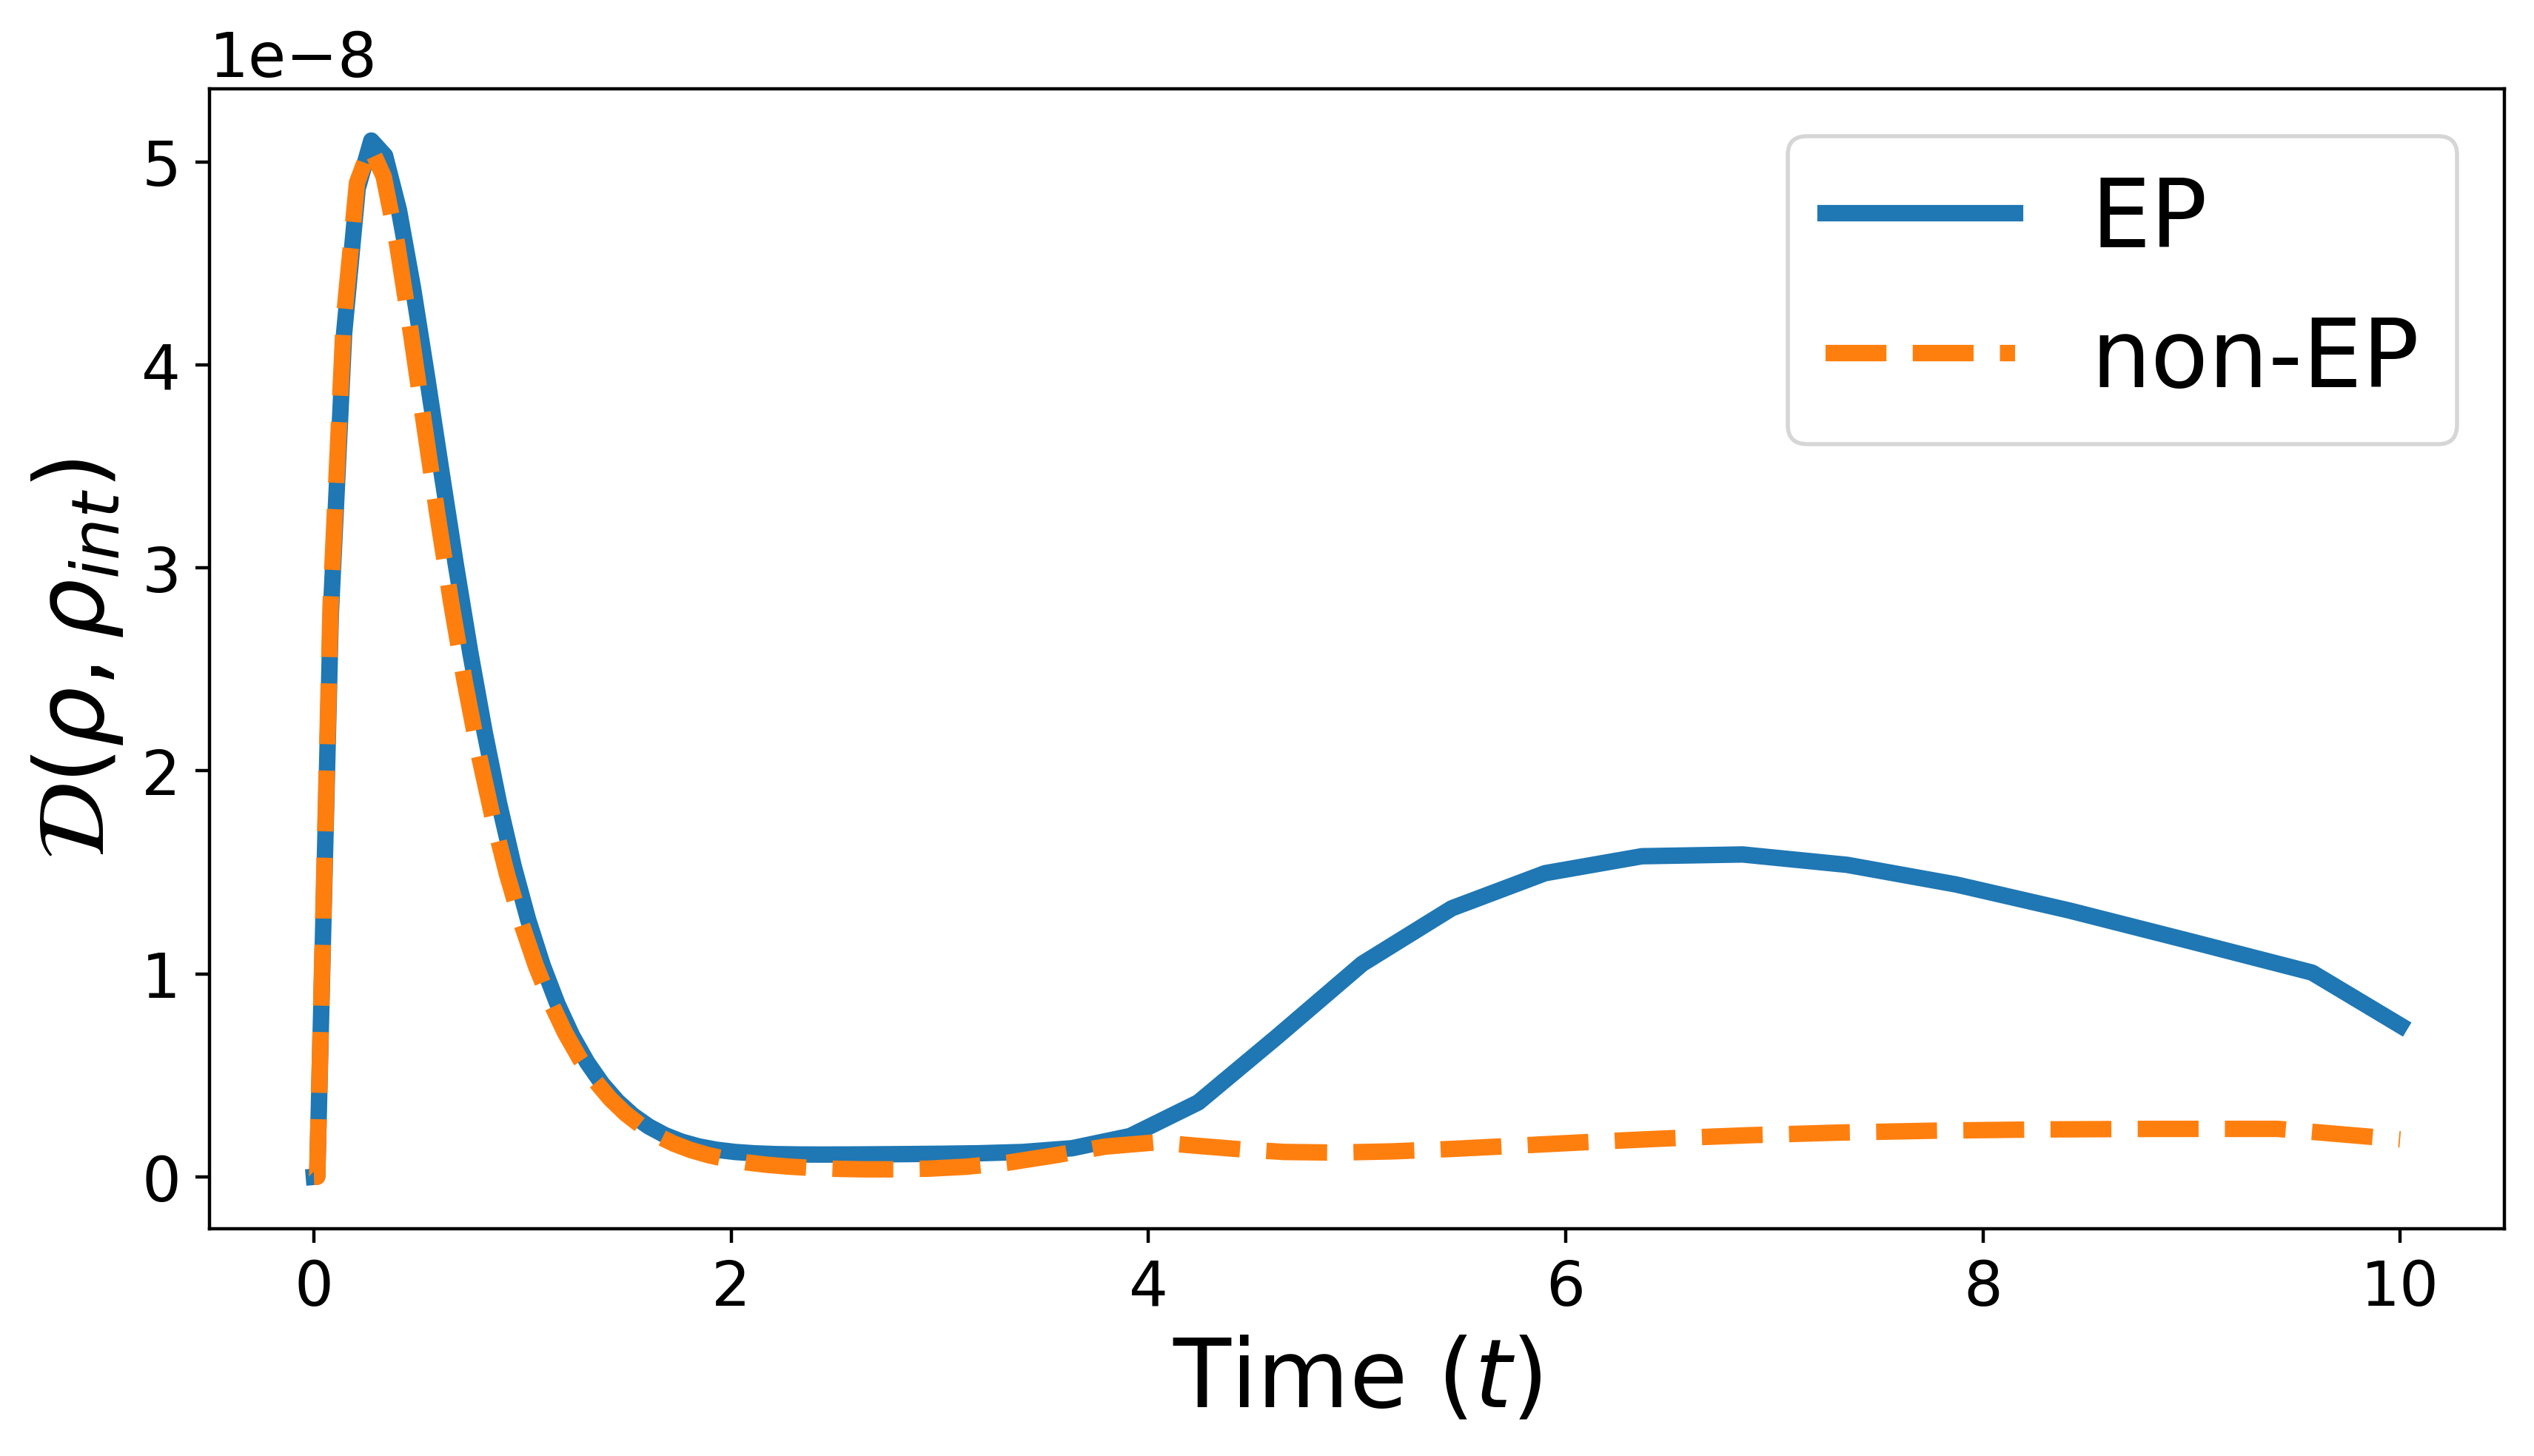
\includegraphics[width=0.6\linewidth]{figures/minevsint.png}
    \caption{The relative distance $\mathcal{D}(\ket{\rho}\rangle, \ket{\rho_\text{int}}\rangle) = ||\ket{\rho}\rangle - \ket{\rho_\text{int}}\rangle||_1/||\ket{\rho_\text{int}}\rangle||_1$ between the density matrices calculated with the implemented methods and with a numerical solver. The two lines represent the distances at the EP and away from the EP, using the corresponding implemented methods for each case. The numerical solver was set to an absolute and relative tolerance of $10^{-10}$ and $10^{-6}$ respectively.}
    \label{fig:minevsint}
\end{figure}

With a clear picture of the analytical dynamics and numerically calculated eigenvalues and generalized eigenvectors at hand, simulations of the parallel dot system could be done. Firstly, the evolution in the generalized modes was investigated. This was done by simulating the density matrix for initial conditions in terms of the generalized eigenvectors, and comparing it with the steady-state of the system, see \cref{fig:diffrho0}.

\begin{figure}[H]
\centering
\begin{subfigure}[t]{.5\textwidth}
  \centering
  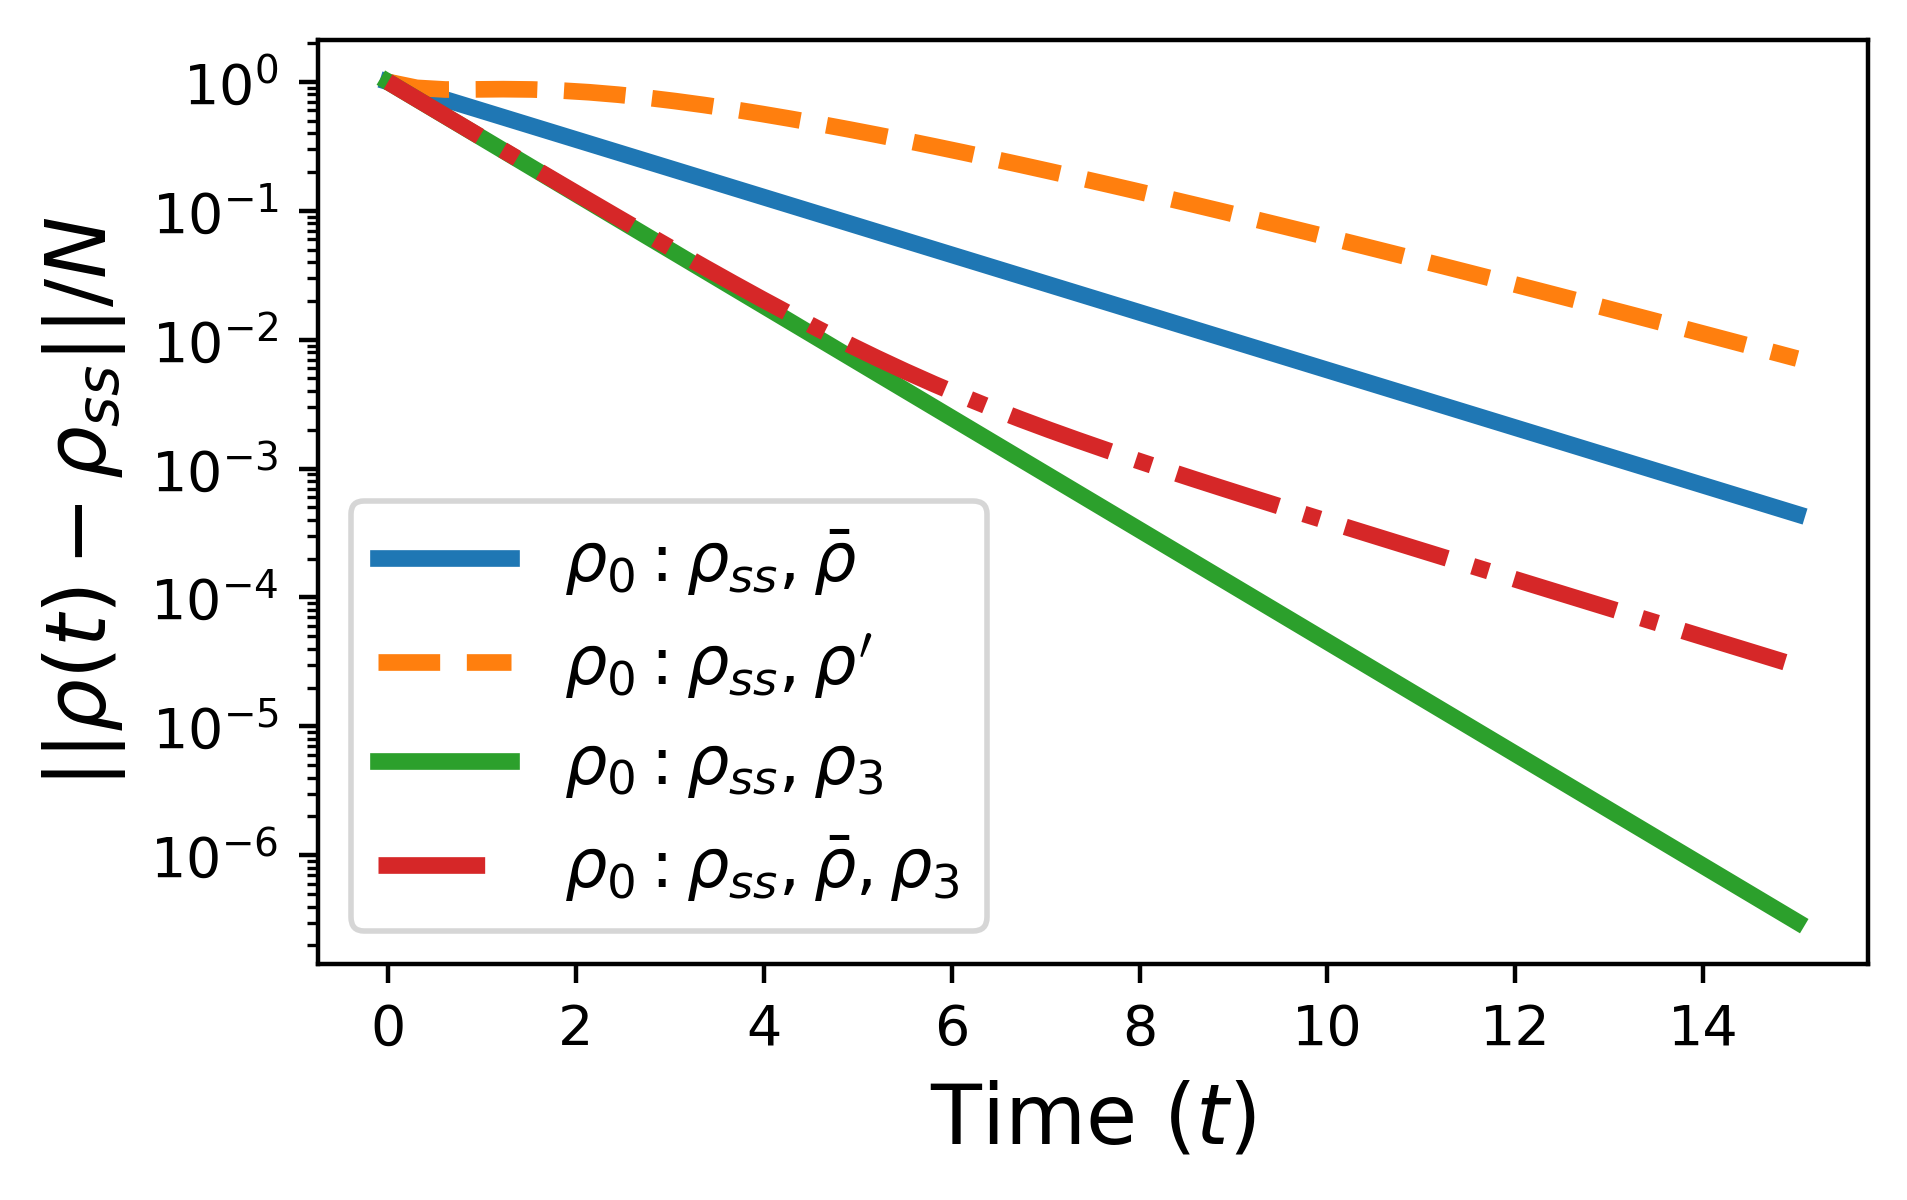
\includegraphics[width=\linewidth]{figures/rho_diff_rho0_v3.png}
  \caption{}
  \label{fig:rhodiffrho0}
\end{subfigure}%
\begin{subfigure}[t]{.5\textwidth}
  \centering
  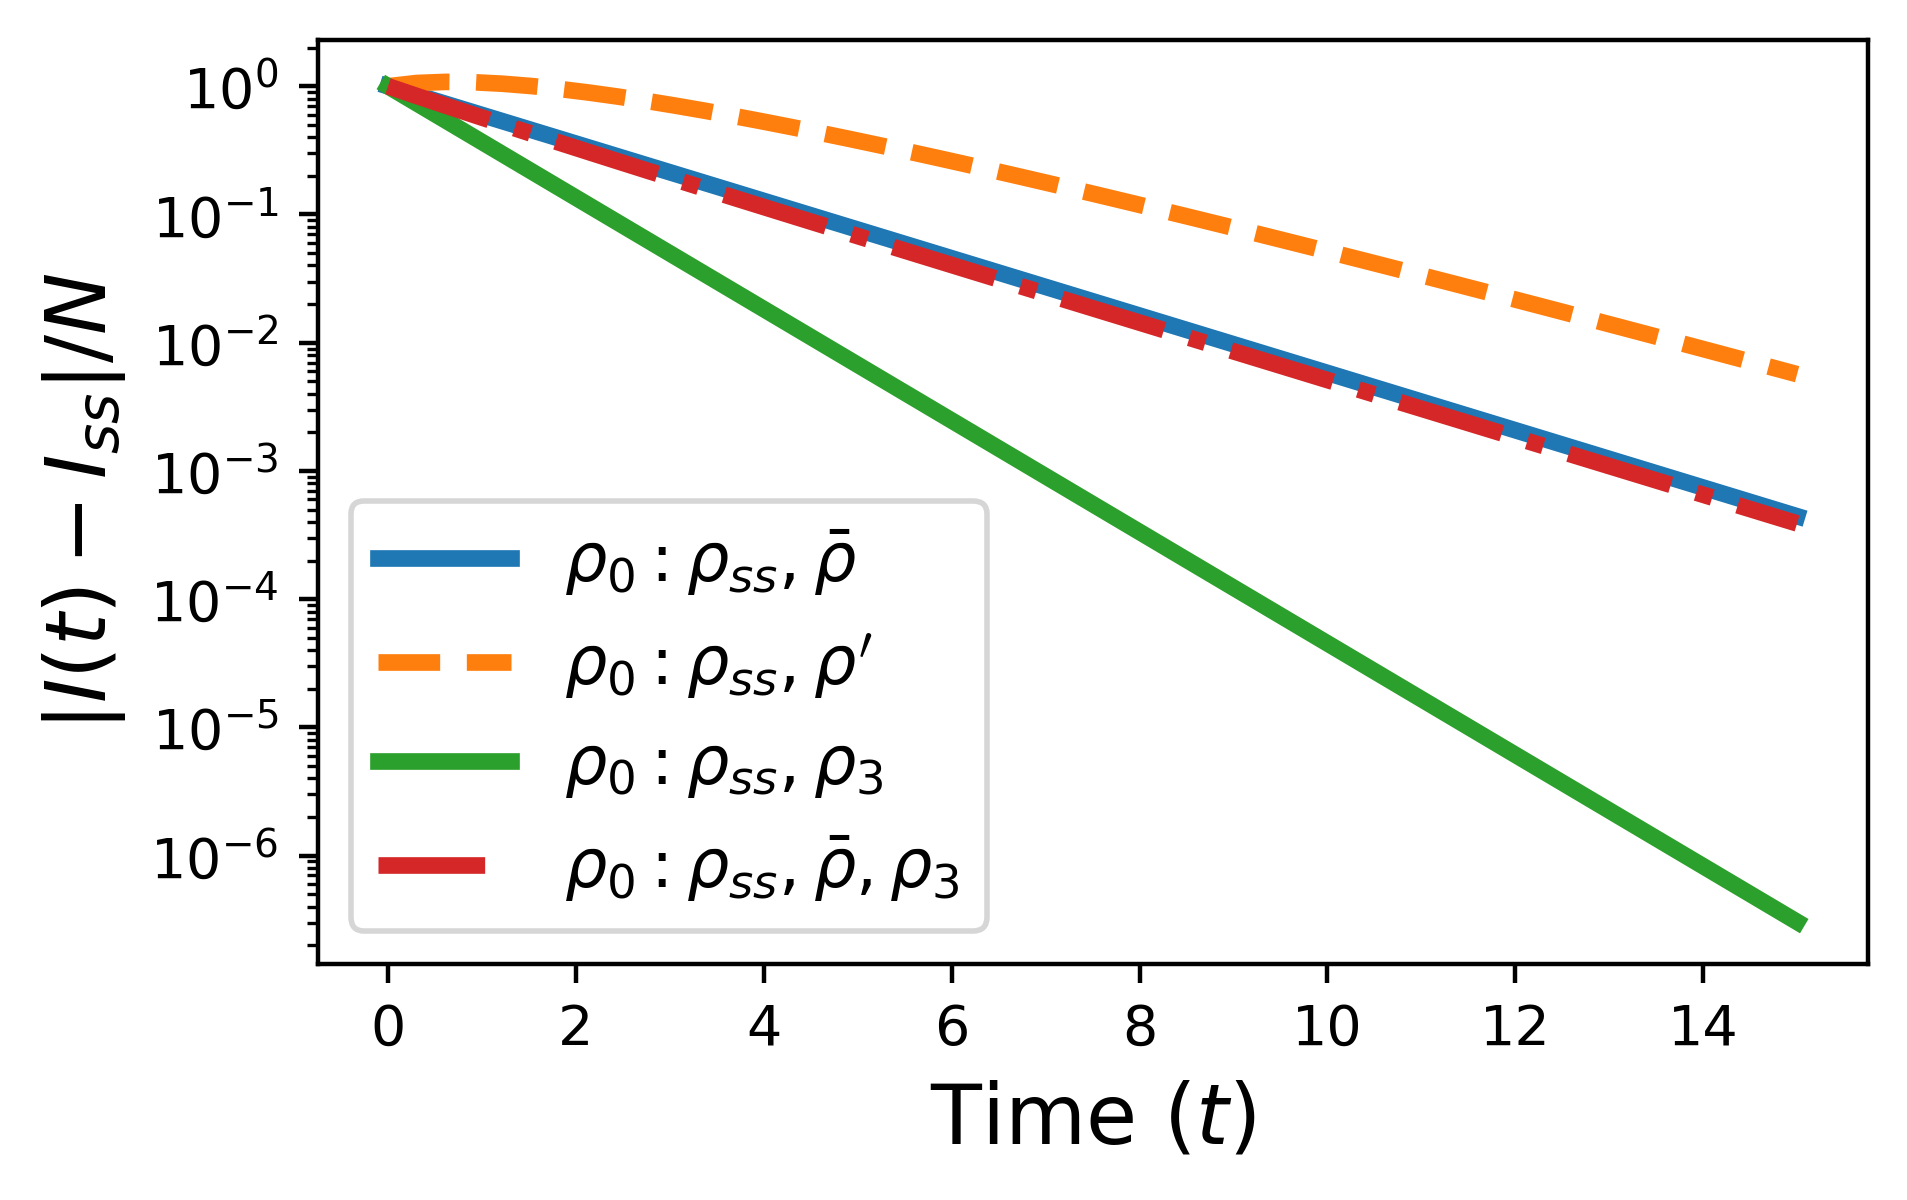
\includegraphics[width=\linewidth]{figures/I_diff_rho0_nonvis.png}
  \caption{}
  \label{fig:Idiffrho0}
\end{subfigure}
\caption{The decay of the density matrix (a) and the current (b), towards the steady state density matrix $\rho_{ss}$ and current $I_{ss}$ in a log plot. The simulations were done at the EP with different initial conditions in terms of the generalized eigenvectors. A normalization by $N=||\rho(0) - \rho_{ss}||$ and $N=||I(0) - I_{ss}||$ was done such that each curve is unity for $t=0$.}
\label{fig:diffrho}
\end{figure}

As discussed in the theory section, any relevant observable of the system can be obtained from the density operator. For the parallel dot system, the main observable is the current $\hat I$, which can be put in terms of the jump operators as follows: 
\begin{equation}
    something
\end{equation}
Using \cref{eq:expec}, the current could then be calculated with $\braket{\hat I}(t) = \tr{(\hat \rho(t)\hat I)}$. Implementing this numerically, the current through the quantum dot system for varying parameters and initial conditions could be simulated. In \cref{fig:diffde}, the dynamics of the current at and slightly away from the exceptional point was simulated.

\begin{figure}[H]
\centering
\begin{subfigure}[t]{.5\textwidth}
  \centering
  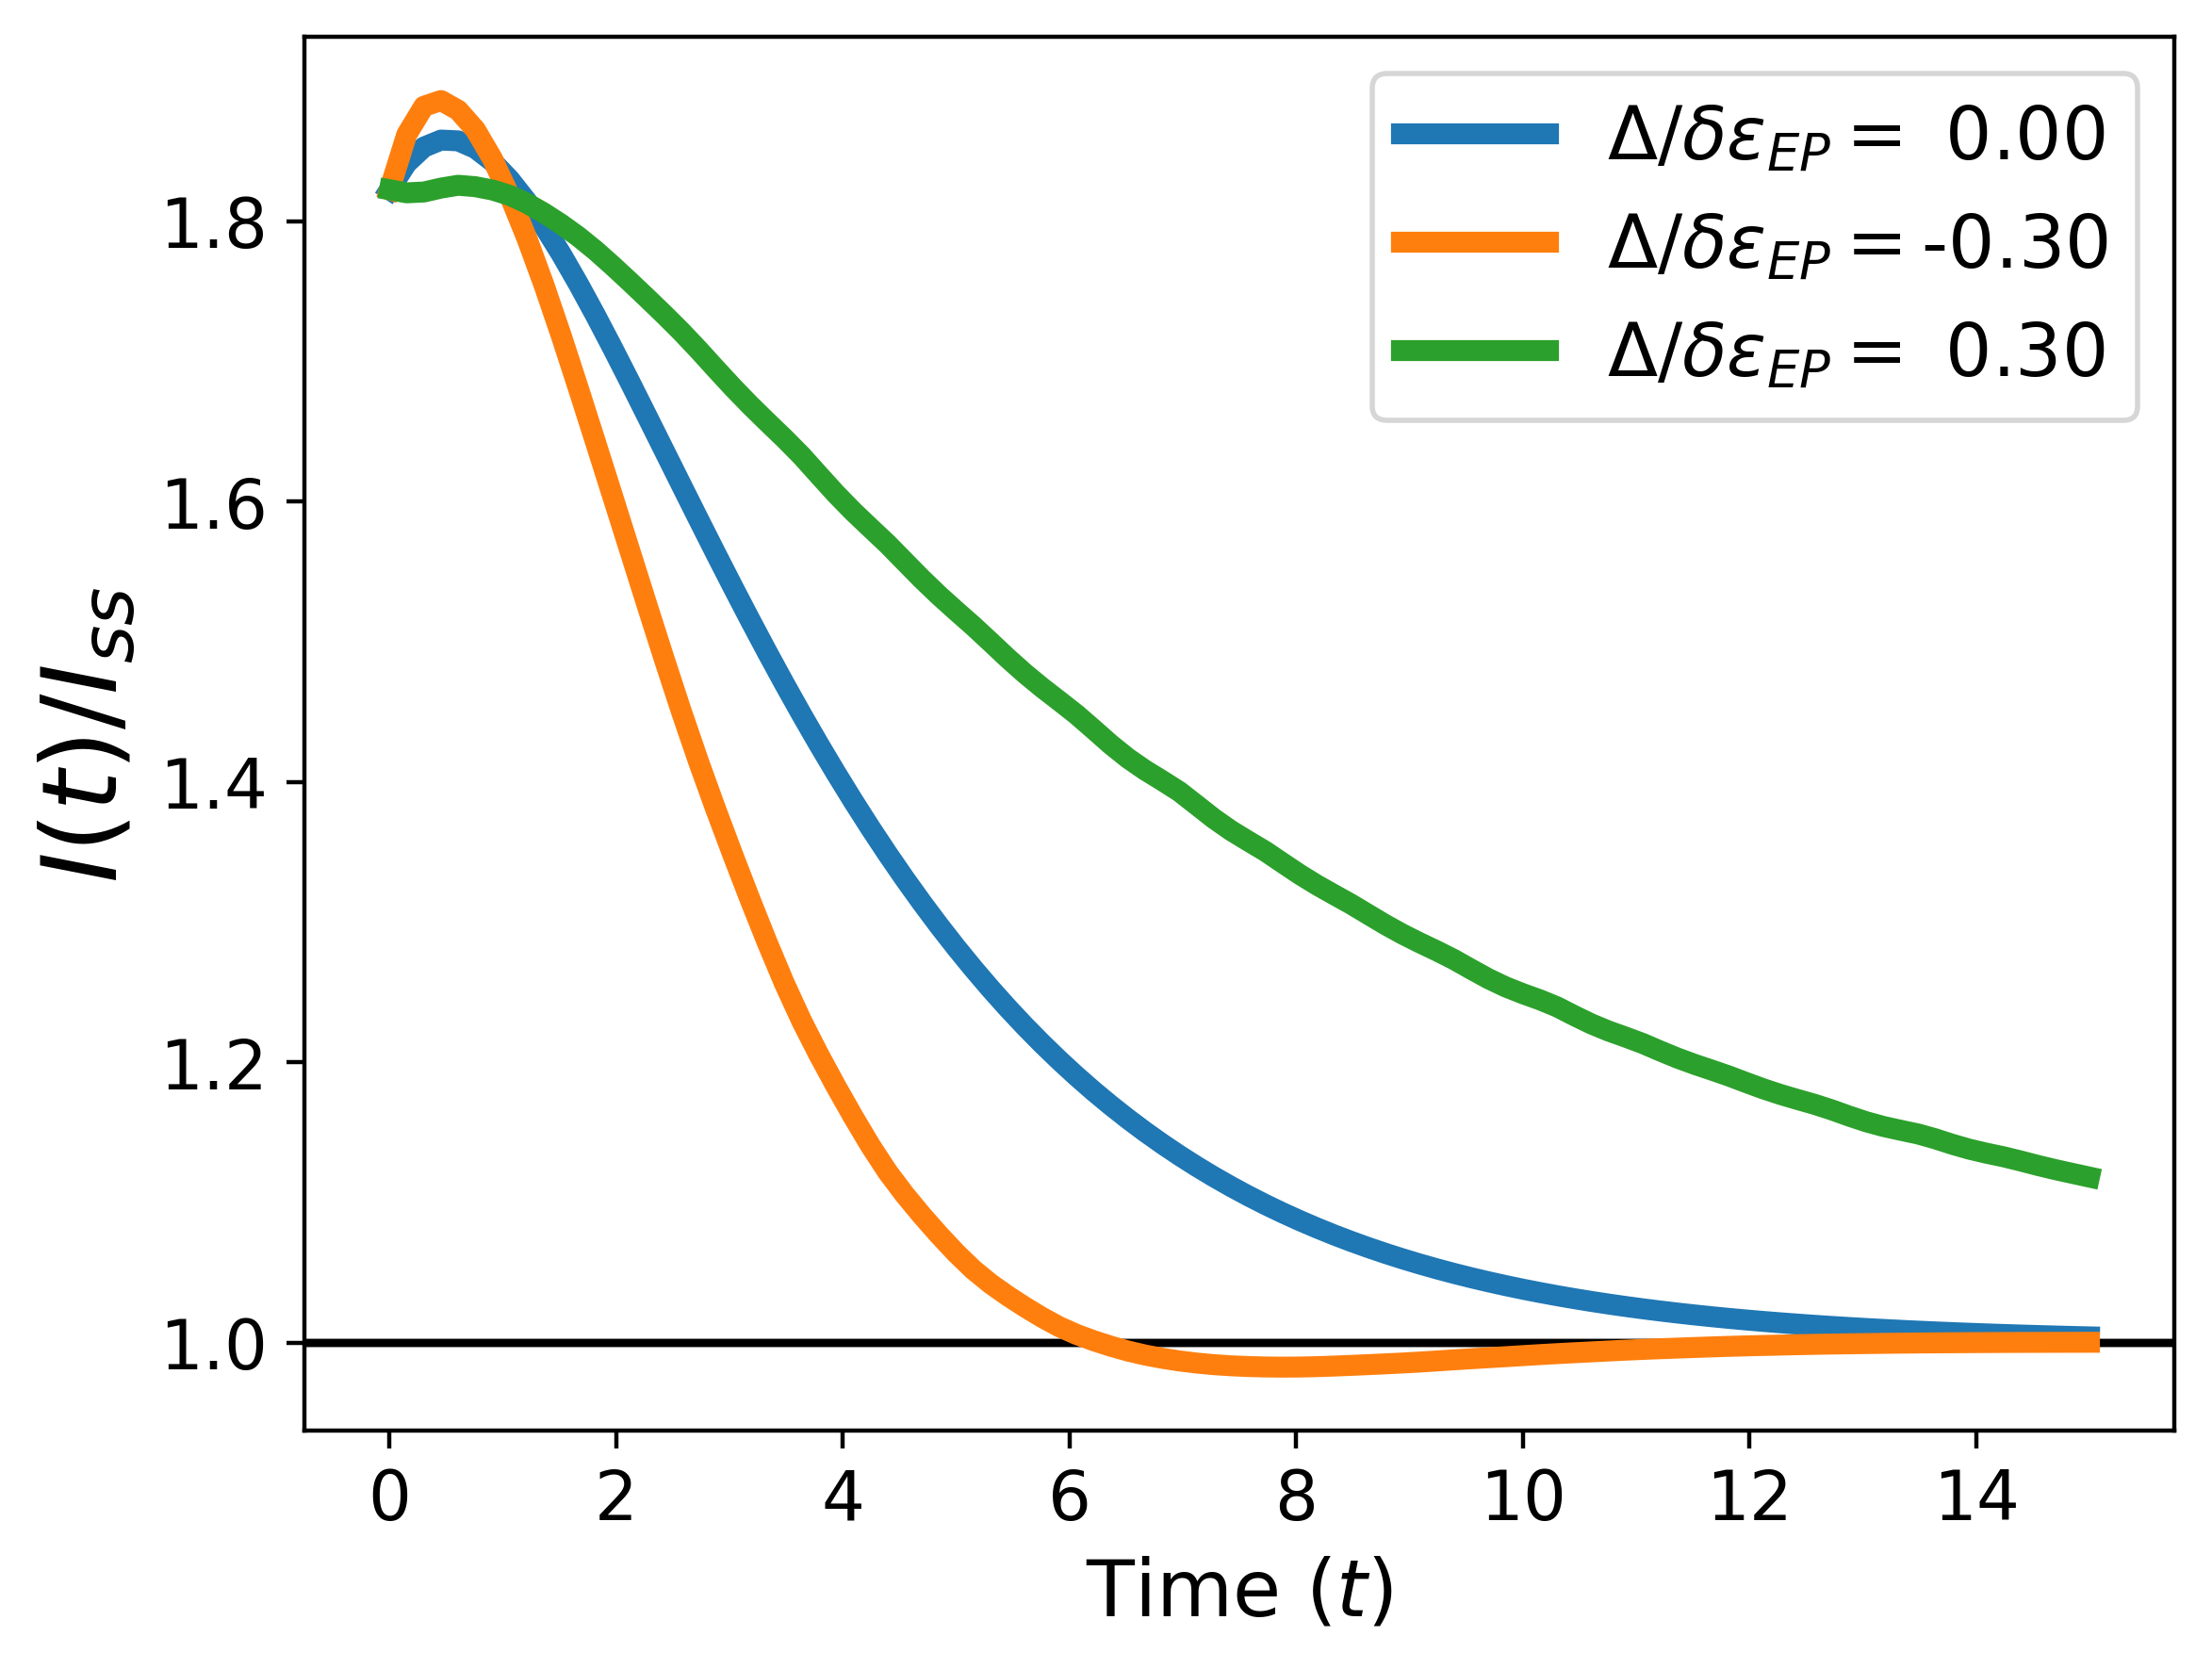
\includegraphics[width=\linewidth]{figures/curr_diff_de.png}
  \caption{}
  \label{fig:diffde1}
\end{subfigure}%
\begin{subfigure}[t]{.5\textwidth}
  \centering
  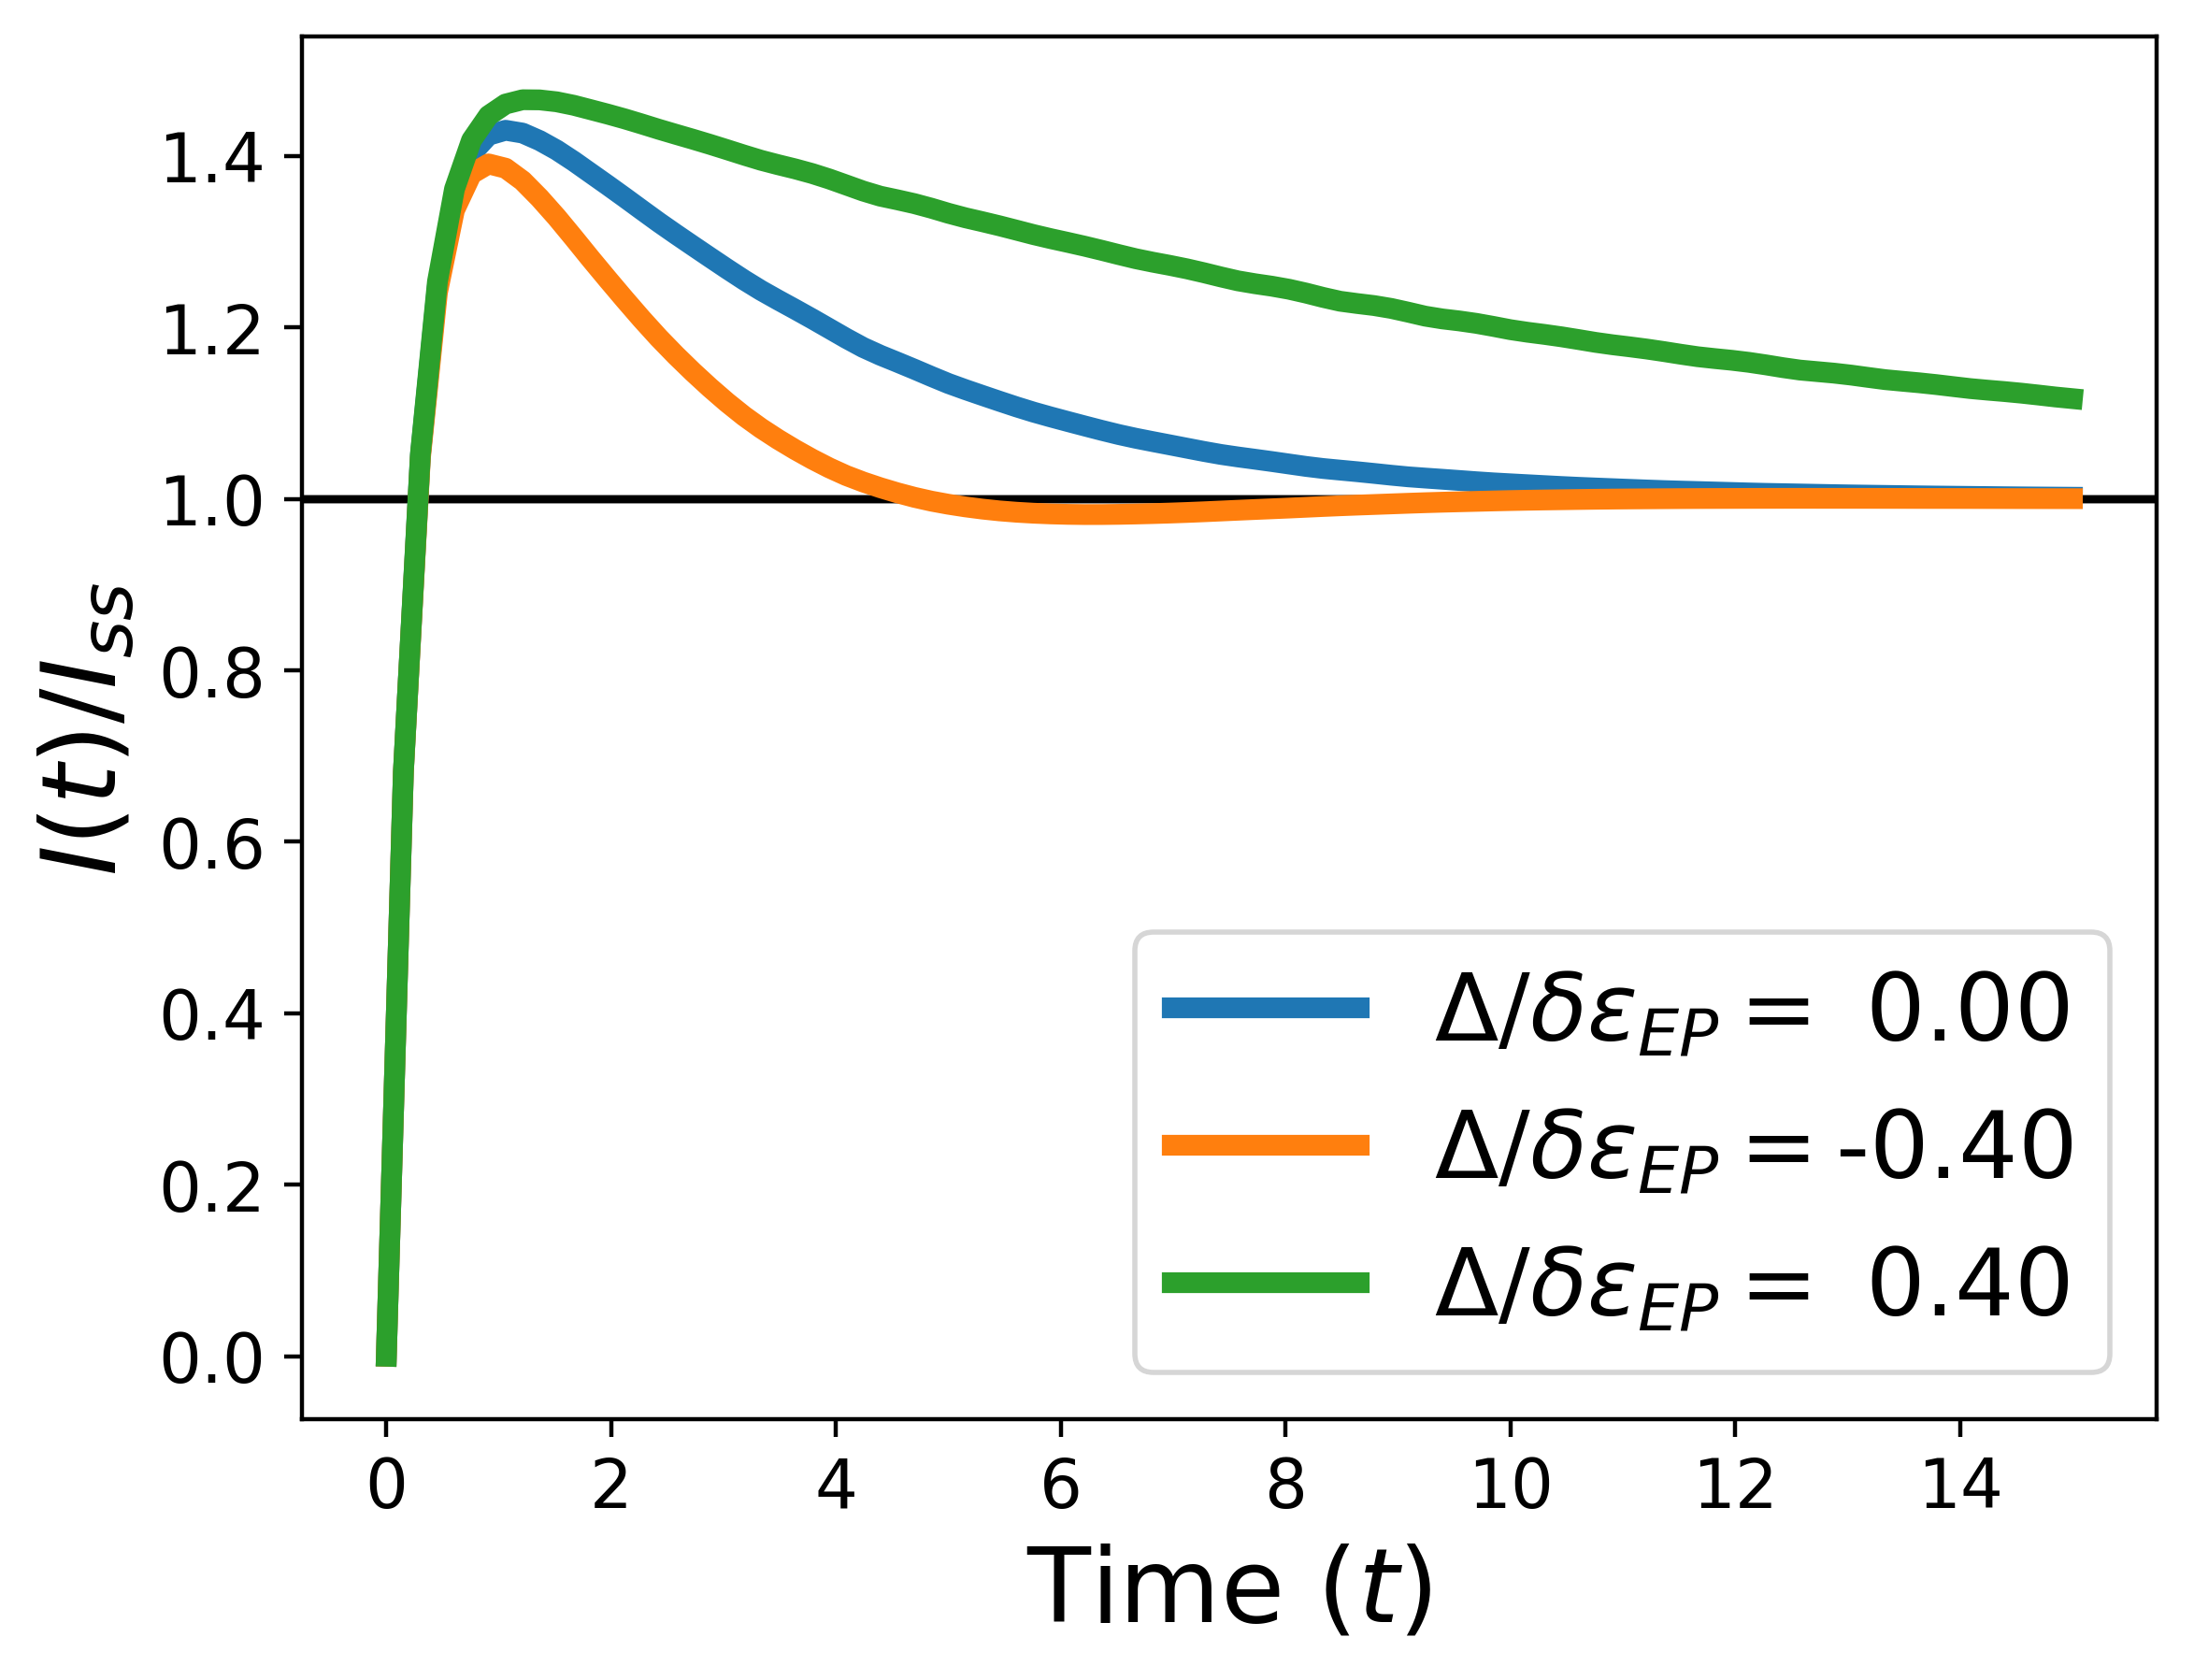
\includegraphics[width=\linewidth]{figures/curr_diff_dev2.png}
  \caption{}
  \label{fig:diffde2}
\end{subfigure}
\caption{The current over time for different $\delta\epsilon$, normalized by the steady state current $I_{ss}$. The solid, blue curve correspond to the system being at the EP, while the other two are slightly away from it.}
\label{fig:diffI}
\end{figure}

% \begin{figure}[H]
%     \centering
%     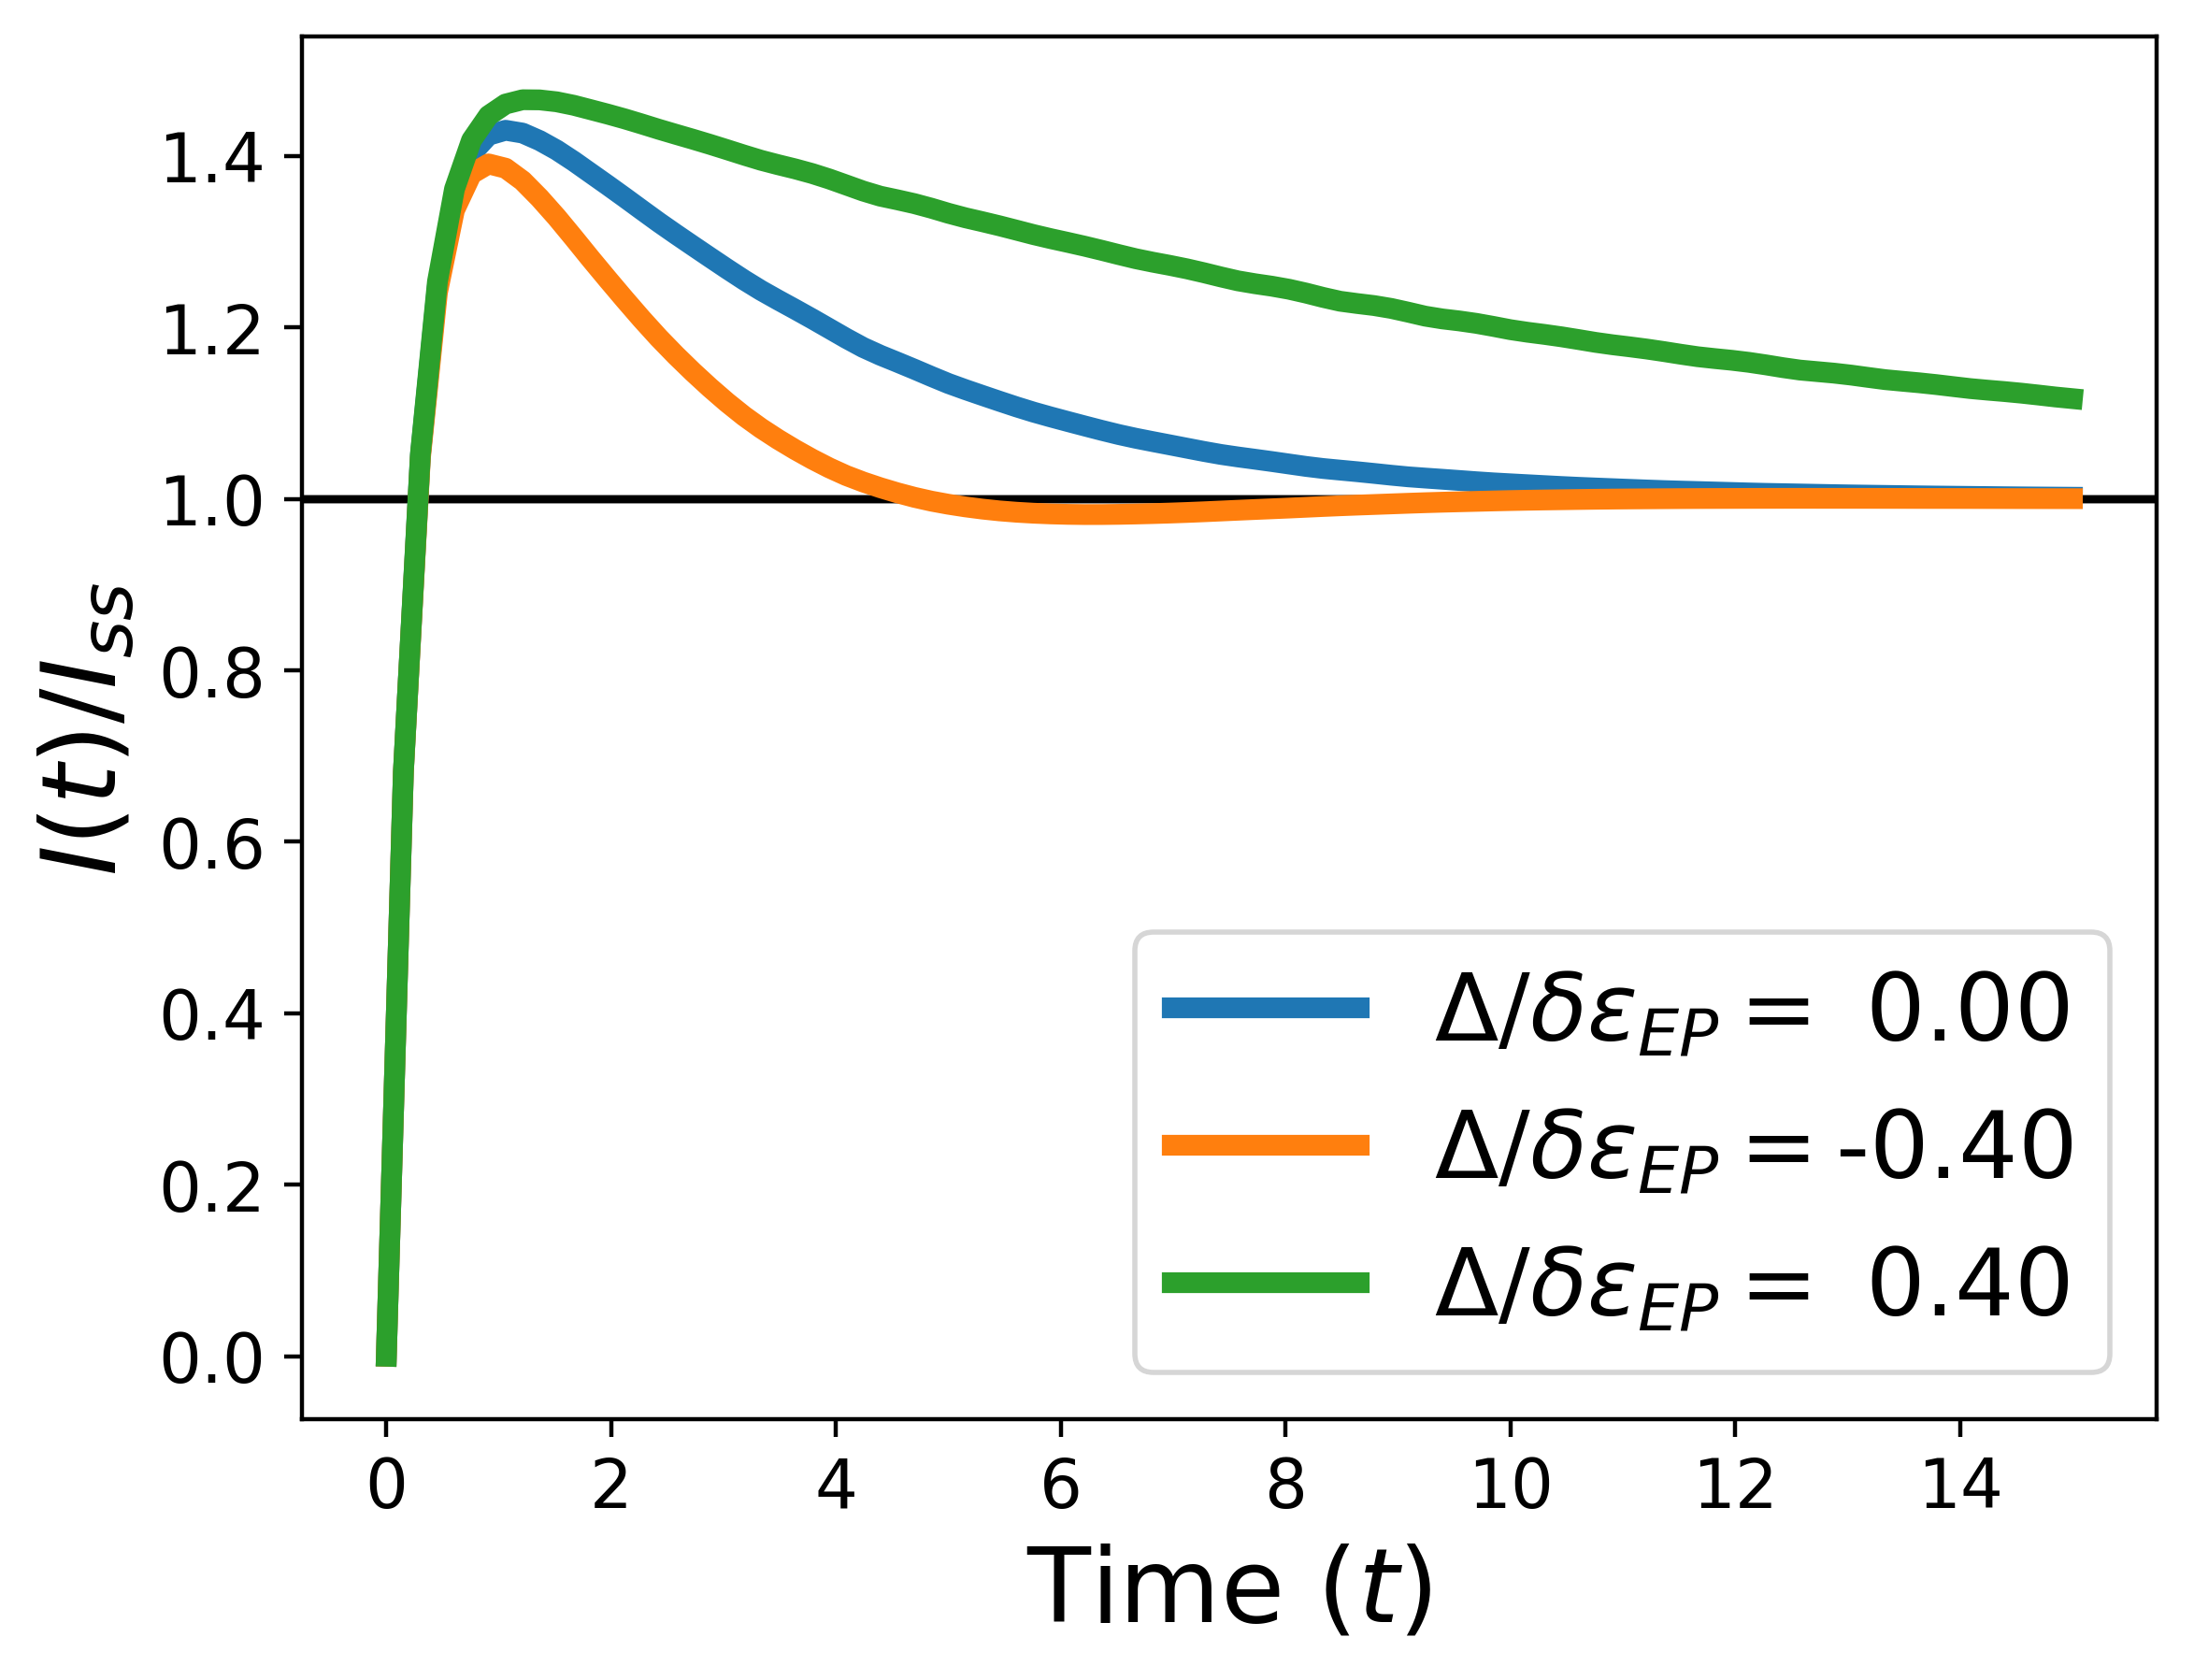
\includegraphics[width=.7\linewidth]{figures/curr_diff_dev2.png}
%     \caption{The current over time for different $\delta\epsilon$, normalized by the steady state current $I_{ss}$. The solid, blue curve correspond to the system being at the EP, while the other two are slightly away from it. All simulations were done with empty dots as initial conditions.}
%     \label{fig:diffde}
% \end{figure}
% \begin{figure}[H]
%     \centering
%     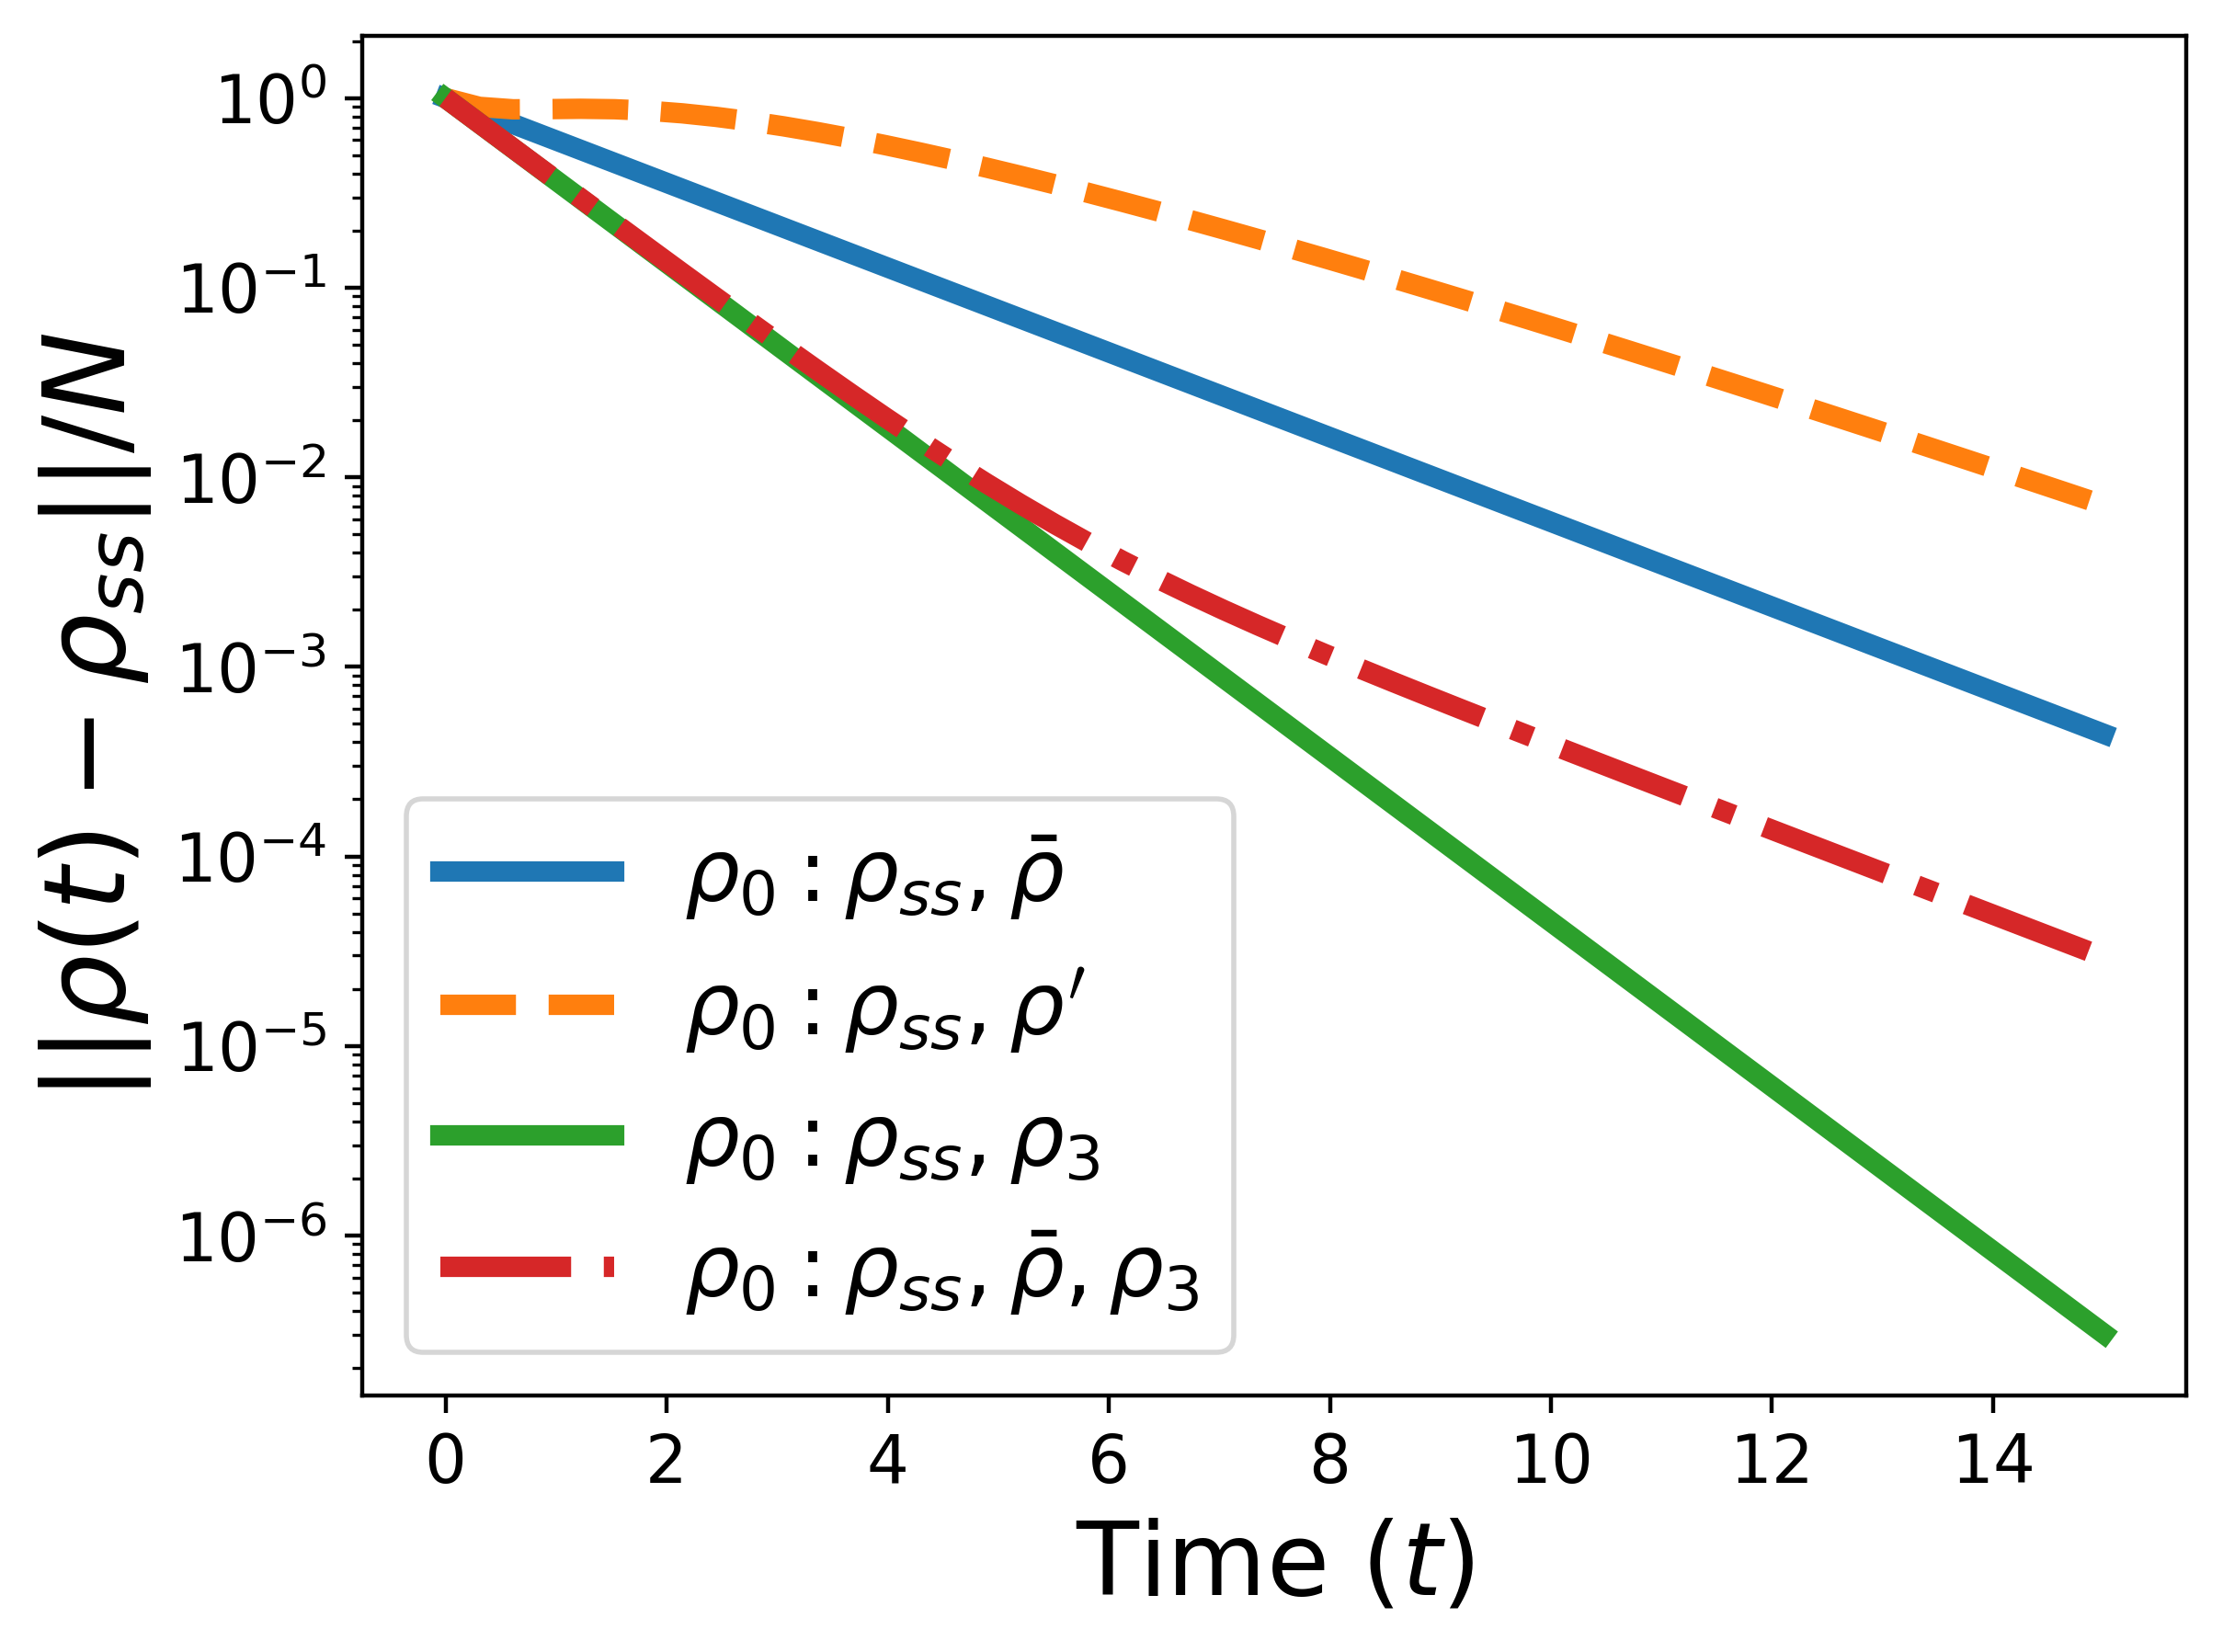
\includegraphics[width=0.5\linewidth]{figures/rho_diff_rho0.png}
%     \caption{The decay of the system towards the steady state $\rho_{ss}$ in a log plot. The simulations were done at the EP with different initial conditions. A normalization by $N=||\rho(0) - \rho_{ss}||$ was done such that each curve is unity for $t=0$.}
%     \label{fig:diffrho0}
% \end{figure}

Add more plots like this with different initial conditions?

\end{document}
